\documentclass{university}

\course{هوش مصنوعی}
\subject{تمرین چهارم بخش دوم}
\professor{دکتر رهبان}

\begin{document}
\allowdisplaybreaks
\setupdocument

\section{}

\subsection{}
زمانی دو متغیر مستقل هستند که هیچ مسیر فعالی بین آن‌ها وجود نداشته باشد. 
پس برای بررسی استقلال هر یک از عبارات داده شده، به دنبال مسیر فعال با فرض 
\lr{shade} 
بودن 
\lr{evidence}ها 
میگردیم. 

\subsubsection{\lr{$P \perp K | W$}}
برقرار نیست. اگر مسیر زرد رنگ شکل 
\ref{fig:1-1-1}
را در نظر بگیریم، این مسیر از یک 
\lr{common effect \footnote{$P \rightarrow W \leftarrow S$}}
و سپس یک 
\lr{cuasal chain \footnote{$S \rightarrow R \rightarrow K$}}
تشکیل شده. پس مسیر فعال است. 

\begin{figure}
    \centering
    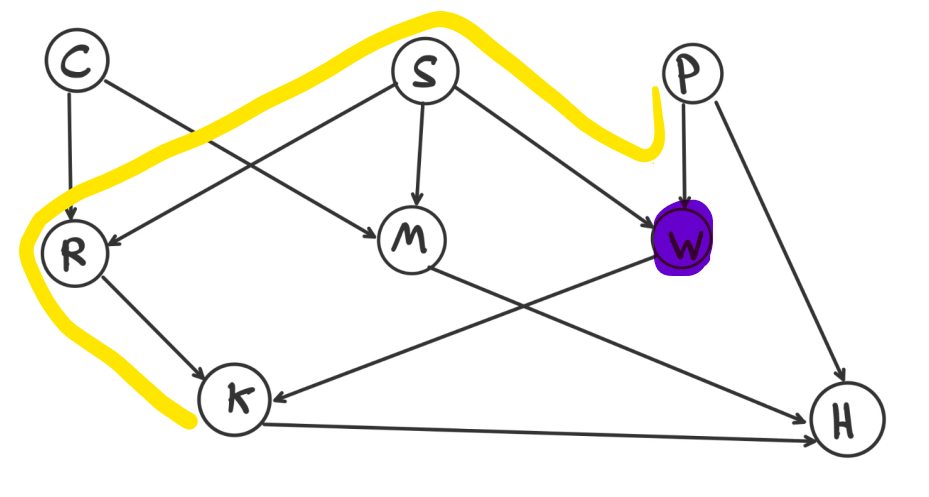
\includegraphics[width=\textwidth]{assets/1-1-1.png}
    \caption{$P \perp K | W$}
    \label{fig:1-1-1}
\end{figure}

\subsubsection{\lr{$P \perp S | K$}}
برقرار نیست. اگر مسیر زرد رنگ شکل 
\ref{fig:1-1-2}
را در نظر بگیریم، این مسیر از یک 
\lr{causal chain \footnote{$P \rightarrow W \rightarrow K$}}
و سپس یک 
\lr{common effect \footnote{$W \rightarrow K \leftarrow R$}}
و بعد یک 
\lr{causal chain \footnote{$S \rightarrow R \rightarrow k$}}
تشکیل شده. پس مسیر فعال است. 

\begin{figure}
    \centering
    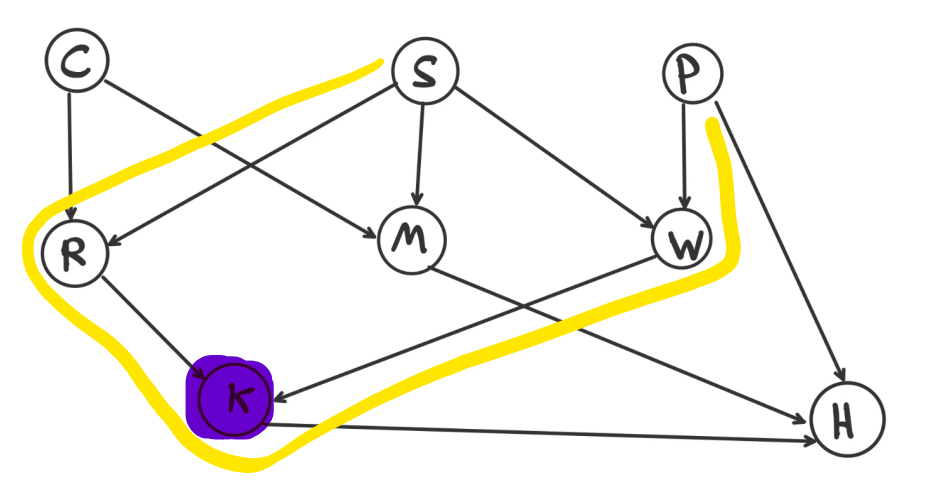
\includegraphics[width=\textwidth]{assets/1-1-2.png}
    \caption{$P \perp S | K$}
    \label{fig:1-1-2}
\end{figure}

\subsubsection{\lr{$P \perp C | H$}}
برقرار نیست. اگر مسیر زرد رنگ شکل 
\ref{fig:1-1-3}
را در نظر بگیریم، این مسیر از یک 
\lr{common effect \footnote{$P \rightarrow H \leftarrow M$}}
و سپس یک 
\lr{cuasal chain \footnote{$C \rightarrow M \rightarrow H$}} 
تشکیل شده. 

\begin{figure}
    \centering
    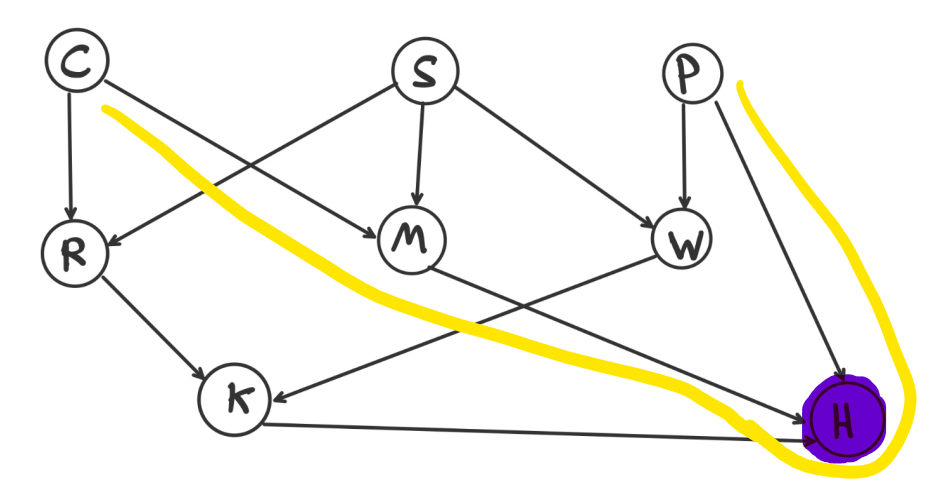
\includegraphics[width=\textwidth]{assets/1-1-3.png}
    \caption{$P \perp C | H$}
    \label{fig:1-1-3}
\end{figure}

\subsection{}
با استفاده از 
\lr{join} و \lr{elimination}
ساده سازی را انجام می‌دهیم. 

\subsubsection{}
\begin{gather*}
    P(R=T) = 0.90484 \times 0.69932 \times 0.70472 \\
    + 0.40307 \times 0.69932 \times 0.29528 \\
    + 0.79326 \times 0.30068 \times 0.70472 \\
    + 0.10731 \times 0.30068 \times 0.29528 \\
    = 0.70677 \\
    P(R=F) = 0.29323 \\
    P(W=T) = 0.80252 \times 0.70472 \times 0.60216 \\
    + 0.89790 \times 0.70472 \times 0.39784 \\
    + 0.09447 \times 0.29528 \times 0.60216 \\
    + 0.30556 \times 0.29528 \times 0.39784 \\
    = 0.64498 \\
    P(W=F) = 0.35502 \\
    P(M=T) = 0.68564 \times 0.69932 \times 0.70472 \\
    + 0.89635 \times 0.69932 \times 0.29528 \\
    + 0.41347 \times 0.30068 \times 0.70472 \\
    + 0.12329 \times 0.30068 \times 0.29528 \\
    = 0.62155 \\
    P(M=F) = 0.37845 \\
    P(K=T) = 0.89633 \times 0.70677 \times 0.64498 \\
    + 0.20737 \times 0.70677 \times 0.35502 \\
    + 0.30714 \times 0.29323 \times 0.64498 \\
    + 0.05066 \times 0.29323 \times 0.35502 \\
    = 0.52398 \\
    P(K=F) = 0.47602 \\
    P(H=T) = 0.95842 \times 0.52398 \times 0.62155 \times 0.60216 \\
    + 0.35837 \times 0.52398 \times 0.62155 \times 0.39784 \\
    + 0.72082 \times 0.52398 \times 0.37845 \times 0.60216 \\
    + 0.30769 \times 0.52398 \times 0.37845 \times 0.39784 \\
    + 0.49234 \times 0.49234 \times 0.62155 \times 0.60216 \\
    + 0.20619 \times 0.49234 \times 0.62155 \times 0.39784 \\
    + 0.42043 \times 0.49234 \times 0.37845 \times 0.60216 \\
    + 0.09646 \times 0.49234 \times 0.37845 \times 0.39784 \\
    = 0.51488
\end{gather*}

\subsubsection{}
\begin{gather*}
    P(H=T|M=T) = 0.95842 \times 0.52398 \times 0.62155 \times 0.60216 \\
    + 0.35837 \times 0.52398 \times 0.62155 \times 0.39784 \\
    + 0.49234 \times 0.49234 \times 0.62155 \times 0.60216 \\
    + 0.20619 \times 0.49234 \times 0.62155 \times 0.39784 \\
    = 0.35021
\end{gather*}

\subsubsection{}
برای حل این قسمت 
\lr{joint ditribution} 
همه متغیرها را بدست می‌آوریم، سپس با حاشیه سازی متغیرهای ناخواسته را حذف می‌کینم. 
پس از آن، با نرمالایز کردن به جواب مطلوب می‌رسیم. 

\begin{gather*}
    P(C, S, P, R, W, M, K, H) \\
    = P(C) P(S) P(P) P(R|C, S) P(W|S, P) P(M|C, S) P(K|R, W) P(H|K, M, P) \\
    P(P=T, S=T, H=T) \\
    = P(P=T, S=T, H=T, C=T, R=T, W=T, M=T, K=T) \\
    + P(P=T, S=T, H=T, C=T, R=T, W=T, M=T, K=F) \\
    + P(P=T, S=T, H=T, C=T, R=T, W=T, M=F, K=T) \\
    + P(P=T, S=T, H=T, C=T, R=T, W=T, M=F, K=F) \\
    + P(P=T, S=T, H=T, C=T, R=T, W=F, M=T, K=T) \\
    + P(P=T, S=T, H=T, C=T, R=T, W=F, M=T, K=F) \\
    + P(P=T, S=T, H=T, C=T, R=T, W=F, M=F, K=T) \\
    + P(P=T, S=T, H=T, C=T, R=T, W=F, M=F, K=F) \\
    + P(P=T, S=T, H=T, C=T, R=F, W=T, M=T, K=T) \\
    + P(P=T, S=T, H=T, C=T, R=F, W=T, M=T, K=F) \\
    + P(P=T, S=T, H=T, C=T, R=F, W=T, M=F, K=T) \\
    + P(P=T, S=T, H=T, C=T, R=F, W=T, M=F, K=F) \\
    + P(P=T, S=T, H=T, C=T, R=F, W=F, M=T, K=T) \\
    + P(P=T, S=T, H=T, C=T, R=F, W=F, M=T, K=F) \\
    + P(P=T, S=T, H=T, C=T, R=F, W=F, M=F, K=T) \\
    + P(P=T, S=T, H=T, C=T, R=F, W=F, M=F, K=F) \\
    + P(P=T, S=T, H=T, C=F, R=T, W=T, M=T, K=T) \\
    + P(P=T, S=T, H=T, C=F, R=T, W=T, M=T, K=F) \\
    + P(P=T, S=T, H=T, C=F, R=T, W=T, M=F, K=T) \\
    + P(P=T, S=T, H=T, C=F, R=T, W=T, M=F, K=F) \\
    + P(P=T, S=T, H=T, C=F, R=T, W=F, M=T, K=T) \\
    + P(P=T, S=T, H=T, C=F, R=T, W=F, M=T, K=F) \\
    + P(P=T, S=T, H=T, C=F, R=T, W=F, M=F, K=T) \\
    + P(P=T, S=T, H=T, C=F, R=T, W=F, M=F, K=F) \\
    + P(P=T, S=T, H=T, C=F, R=F, W=T, M=T, K=T) \\
    + P(P=T, S=T, H=T, C=F, R=F, W=T, M=T, K=F) \\
    + P(P=T, S=T, H=T, C=F, R=F, W=T, M=F, K=T) \\
    + P(P=T, S=T, H=T, C=F, R=F, W=T, M=F, K=F) \\
    + P(P=T, S=T, H=T, C=F, R=F, W=F, M=T, K=T) \\
    + P(P=T, S=T, H=T, C=F, R=F, W=F, M=T, K=F) \\
    + P(P=T, S=T, H=T, C=F, R=F, W=F, M=F, K=T) \\
    + P(P=T, S=T, H=T, C=F, R=F, W=F, M=F, K=F) \\
    = P(P=T) P(S=T) P(H=T|K=T, M=T, P=T)\\ P(C=T) P(R=T|C=T, S=T) P(W=T|S=T, P=T)\\ P(M=T|C=T, S=T) P(K=T|R=T, W=T) \\
    + P(P=T) P(S=T) P(H=T|K=F, M=T, P=T)\\ P(C=T) P(R=T|C=T, S=T) P(W=T|S=T, P=T)\\ P(M=T|C=T, S=T) P(K=F|R=T, W=T) \\
    \vdots \\
    + P(P=T) P(S=T) P(H=T|K=F, M=F, P=T)\\ P(C=F) P(R=F|C=F, S=T) P(W=F|S=T, P=T)\\ P(M=F|C=F, S=T) P(K=F|R=F, W=F) 
\end{gather*} 

اعداد را از جدول جایگذاری کنیم جواب به دست آمده را نرمالایز کنیم، جواب نهایی بدست می‌آید.

\end{document}